\section{Maximal Series-Parallel Graphs}\label{section:SP-graphs}

Maximal series-parallel graphs correspond to the class of 2-trees \cite[P. 2]{straight-line_2-trees} and are a suitable class of interest for fundamental research since any 2-tree is biconnected, but not triconnected and inherits a constant treewidth. Since maximal SP-graph contains a largest maximal outerplanar subgraph, creating a compact layered polyline drawing for maximal outerplanar graphs described in section \ref{s:maximal_outerplanar} will prove to be useful when drawing maximal SP-graphs. 

\subsection{Properties Of Maximal Series Parallel Graphs}

% 2-tree stuff

\begin{lemma}
	There exists a linear time algorithm which computes the largest maximal outerplanar subgraph for any maximal SP-graph.
\end{lemma}
\begin{proof}
	Consider the tree decomposition $(T,W)$ of $G$. Add the root of $T$ to $T'$ and its bag to $W'$. From the root of $T$, pick the three children which root the subtrees with the maximum height and size and their respective bags. Then, recursively pick the two children which root the subtrees with the maximum height and size and add them to $T'$ with their respective bags to $W'$. This procedure terminates some leaves of $T$.\\
	Every vertex of the resulting $T'$ is of degree maximum 3 and by Lemma \ref{l:outerplanar_tree_decomposition}, the graph $G'$ induced by $T$ is maximal outerplanar. Since during this procedure, the nodes with the maximum subtrees are chosen and the properties described in Lemma \ref{l:outerplanar_TD_properties} hold, there exists no other maximal outerplanar subgraph of $G$ which is larger. 
\end{proof}

\begin{lemma}
	Let $G$ be a maximal SP-graph with tree decomposition $(T,W)$ and $G'$ any maximal SP subgraph of $G$ with tree decomposition $(T',W')$. Then, it holds:
	\begin{enumerate}
		\item $(T',W') \subseteq (T,W)$
		\item There exists a vertex in $T\setminus T'$ whose bag shares exactly two vertices of $G$ with the bag of the root of $T'$
	\end{enumerate}
\end{lemma}	
\begin{proof}
	\begin{itemize}
		\item Since the tree decomposition of a maximal SP-graph is unique, any maximal SP subgraph $G'$ of $G$ is represented in $T$ by $T'$.
		\item Let $t$ be the root of $T'$. Consider the parent of $t$ in $T$. Then, by Lemma \ref{l:outerplanar_two_vertices_subtree_TD_2}, $t$ and its parent share two vertices in their respective bags.
	\end{itemize}
\end{proof}

% drawing stuff

\subsection{Drawing Algorithm For Maximal Series Parallel Graphs With Two Bends}

A maximal SP-graph $G$ with its tree decomposition $(T,W)$ will be evaluated for its largest maximal outerplanar subgraph $G'$ with tree decomposition $(T',W')$. $\tilde{T}$ describes the difference of $T$ and $T'$ and is a set of subtrees of $T$.\\
In order to create a polyline drawing similarily as described in section \ref{s:maximal_outerplanar}, it is crucial to find a suiting $SPQR$-Tree derivation of a maximal SP-graphs for the box drawing algorithm \ref{al:draw_SPQR} to function. Fortunately, the function deriving a $SPQR$-Tree of a tree decomposition of a maximal outerplanar graph $G'$ is also applicable for maximal SP-graphs.
\begin{lemma}
	The function deriving a $SPQR$-Tree from a tree decomposition defined in Lemma \ref{l:tree_decomp_to_SPQR} is applicable to any maximal SP-graph $G$.
\end{lemma}
\begin{proof}
	Let $G$ be a maximal SP-graph with its tree decomposition $(T,W)$. Contrary to a tree decomposition of a maximal outerplanar graph, any node $T$ can have arbitrary many children. Inserting a new vertex described with a vertex in $T$ works analogously to the prior scheme. For a maximal SP-graph, the resulting $SPQR$-Tree can inherit arbitrary many serial nodes attached to a parallel node.
\end{proof}

After $(T',W')$ is drawn into a box drawing $B'$, the remaining subtrees in $\tilde{T}$ will be inserted accordingly, resulting in a box drawing $B$ for $G$. Finally, a polyline drawing will be derived from $B$.

\begin{lemma}
	Let $G$ be a maximal SP-graph and $G'$ its largest maximal outerplanar graph with its box drawing $\mathcal{B}_{G'}$ created by Algorithm \ref{al:maximal_outerplanar_box_two_bends}. For every tree $t$ in $\tilde{t}$ there exists a column in $\mathcal{B}_{G'}$ where $t$ can be inserted into without destroying planarity. 
\end{lemma}
\begin{proof}
	Consider the two shared vertices $u,l \in G$ of the root of $t$ with its parent. Since the parent of $t$ is part of $G'$, $u$ and $l$ are placed on their respective layers in $\mathcal{B}_{G'}$ and connected by an edge at column $x$ with its content drawn from $G'$. Insert $t$ by slicing the box drawing so that there are sufficient free columns beginning at $x+1$ and draw $t$. This way, planarity is preserved. 
	
	\begin{figure}[H]
	\centering
	\begin{subfigure}{\textwidth}
		\centering
		\includegraphics[page=2,width=0.6\linewidth]{graphics/t_insertion_into_maximal_outerplanar.pdf}
		\caption{$t$ inserted inbetween upper and lower layer $u$ and $l$ (colored in orange)}
	\end{subfigure}
	
\end{figure}
	
\end{proof}

\begin{algorithm}[H]
	\KwIn{Maximal Series Parallel Graph $G$}
	\KwOut{Polyline Drawing $\Gamma_G$ with two bends per edge}
	\caption{\texttt{DrawMaximalSPGraph}$(G)$}\label{al:DrawMaximalSPGraph}
	$(T,W) \gets$ tree decomposition of $G$\\
	$G' \gets$ largest maximal outerplanar subgraph of $G$\\
	$(T',W') \gets$ tree decomposition of $G'$\\
	$\tilde{T} \gets T\setminus T'$\\
	$\Gamma_{G'} \gets \texttt{DrawMaximalOuterplanar}(G')$\\
	\For{$t\in \tilde{T}$}{
		 $p \gets \texttt{parent}(t\texttt{.root})$\\
		 $u \gets \Gamma_{G'}\texttt{.upperLayer}(p)$\\
		 $l \gets \Gamma_{G'}\texttt{.lowerLayer}(p)$\\
		 $\Gamma_{G'}\texttt{.Insert}(t, u, l)$
	}
	\Return $\Gamma_{G'}$
\end{algorithm}

\subsubsection{Analysis}

\begin{lemma}
	When the remaining subtrees of $\tilde{t}$ are inserted into a box drawing $\mathcal{B}_{G'}$, the area bounds do not increase asymptotically.\label{l:SP_not_increasing_area}
\end{lemma}
\begin{proof}
	Let $G$ be a maximal SP-graph with $\mathcal{B}_{G'}$ a box drawing from the largest maximal outerplanar graph of $G$ created by Algorithm \ref{al:maximal_outerplanar_box_two_bends}. For the insertion of $t\in \tilde{t}$ into $\mathcal{B}_{G'}$, consider the subtrees adjacent to the parent $p$ of $t$ in $T$. Since $t$ is not in $T'$, there exists subtree $t'$ of $T'$ adjacent to $p$ which was already drawn.\\
	If the insertion of a tree $t$ would create more layers than drawing $t'$ in the first place resulting in a new upper bound for the height of the drawing, then there would be a maximal outerplanar subgraph of $G$ containing $t'$ which is contradicting the assumption. In the width of the drawing, there are still as many columns as there are edges in $G$. The area bounds do not increase asymptotically.
\end{proof}

% Results

\begin{theorem}
	Any maximal SP-graph admits a polyline drawing in $\mathcal{O}(n^2 \log^2 n)$ area with two bends per edge and a ratio bound by $\mathcal{O}(\log^2 n)$, when the minimal distance between two layers is set to $n$. \label{th:maximal_SP-n^2log^2n-area}
\end{theorem}
\begin{proof}
	Let $\mathcal{B}_{G'}$ be the box drawing of the largest maximal outerplanar subgraph $G'$ of a maximal SP-graph $G$. The width of $\mathcal{B}_{G'}$ lies in $\mathcal{O}(n')$. Inserting the remaining subtrees of $\tilde{t}$ increases the width asymptotically to $\mathcal{O}(n)$ since there is at most one column per edge of $G$. Lemma \ref{l:SP_not_increasing_area} states that the height bound is asymptotically not altered and analogously to the proof of theorem \ref{th:maximal_outerplanar_log2_n_ratio}, the ratio of the resulting polyline drawing $\Gamma_G$ is bound by the amount of total layers, when the minimal distance is set to $n$.
\end{proof}
\begin{theorem}
	Any SP-graph $G$ admits a polyline drawing in $\mathcal{O}(n^2 \log^2 n)$ area with two bends per edge and a ratio bound by $\mathcal{O}(\log^2 n)$, when the minimal distance between two layers is set to $n$.
\end{theorem}
\begin{proof}
	Insert marked edges until $G$ is a maximal SP-graph. Draw $G$ with algorithm \ref{al:DrawMaximalSPGraph} and by theorem \ref{th:maximal_SP-n^2log^2n-area}, the area and ratio upper bounds hold. Removing the marked edges again does not alter any of the upper bounds.
\end{proof}


\begin{theorem}
	Any maximal SP-graph admits a polyline drawing in $\mathcal{O}(n \log^2 n)$ area with two bends per edge.
\end{theorem}
\begin{proof}
	When the minimal distance between two layers is set to a constant, the resulting height is bounded by the amount of simultaneously active vertices. By Lemma \ref{l:maximal_outerplanar_log2_n_vercies_active} and \ref{l:SP_not_increasing_area}, the height is bounded by $\mathcal{O}(\log^2 n)$. The width is still bounded by the amount of edges and the total area consumption lies in $\mathcal{O}(n \log^2 n)$.
\end{proof}


\begin{theorem}
	Any SP-graph admits a polyline drawing in $\mathcal{O}(n \log^2 n)$ area with two bends per edge.
\end{theorem}
\begin{proof}
	Insert marked edges until $G$ is a maximal SP-graph. Draw $G$ with algorithm \ref{al:DrawMaximalSPGraph} and a constant distance between the layers. Afterwards, remove the marked edges from the drawing.
\end{proof}

\subsubsection{Generalization To Planar 3-trees?}
Following the recursive definition of $k$-trees, 3-trees start with a $K_4$ and every new added vertex is connected to three adjacent vertices. 3-trees inherit a treewidth of 3 and $R$ nodes in the respective $SPQR$ tree since they are triconnected. The box drawing algorithm \ref{al:draw_SPQR} does not suffice for this class of planar graphs since the algorithm does not handle the $R$ node case. Still, it is of interest how the idea of a layered box drawing approach will work out based on the tree decomposition of a 3-tree.

\begin{definition}
	Let $G$ be a 3-tree with its tree decomposition $(T,W)$. $G$ is called \emph{complete}, if the following property holds:
	\begin{itemize}
		\item Every vertex of $T$ is either a leaf or of degree 4
		\item The leaves of $T$ have uniform heights
	\end{itemize}
	In other words, $G$ is called complete if the root of $T$ is the parent of 4 complete tertiary trees of the same height.
\end{definition}

\begin{observation}
	Let $G$ be a complete 3-tree. Applying a layering scheme similar to algorithm \ref{al:complete_outerplanar}, the resulting box drawing $\mathcal{B}_G$ is at least in area bound $\mathcal{O}(n^2)$, when the minimal distance between layers is set to a constant.
\end{observation}

In order validate this observation, a box drawing of $K_4$ is created as illustrated. $K_4$ represents the root of the tree decomposition of a complete 3-tree $G$ with height 0 in its tree decomposition $T$. Let $\mathcal{L}_0$ be the list of layers consisting of the topmost and bottommost layer of the $K_4$ for $h=0$.

\begin{figure}[H]
	\centering
	\begin{subfigure}{\textwidth}
		\centering
		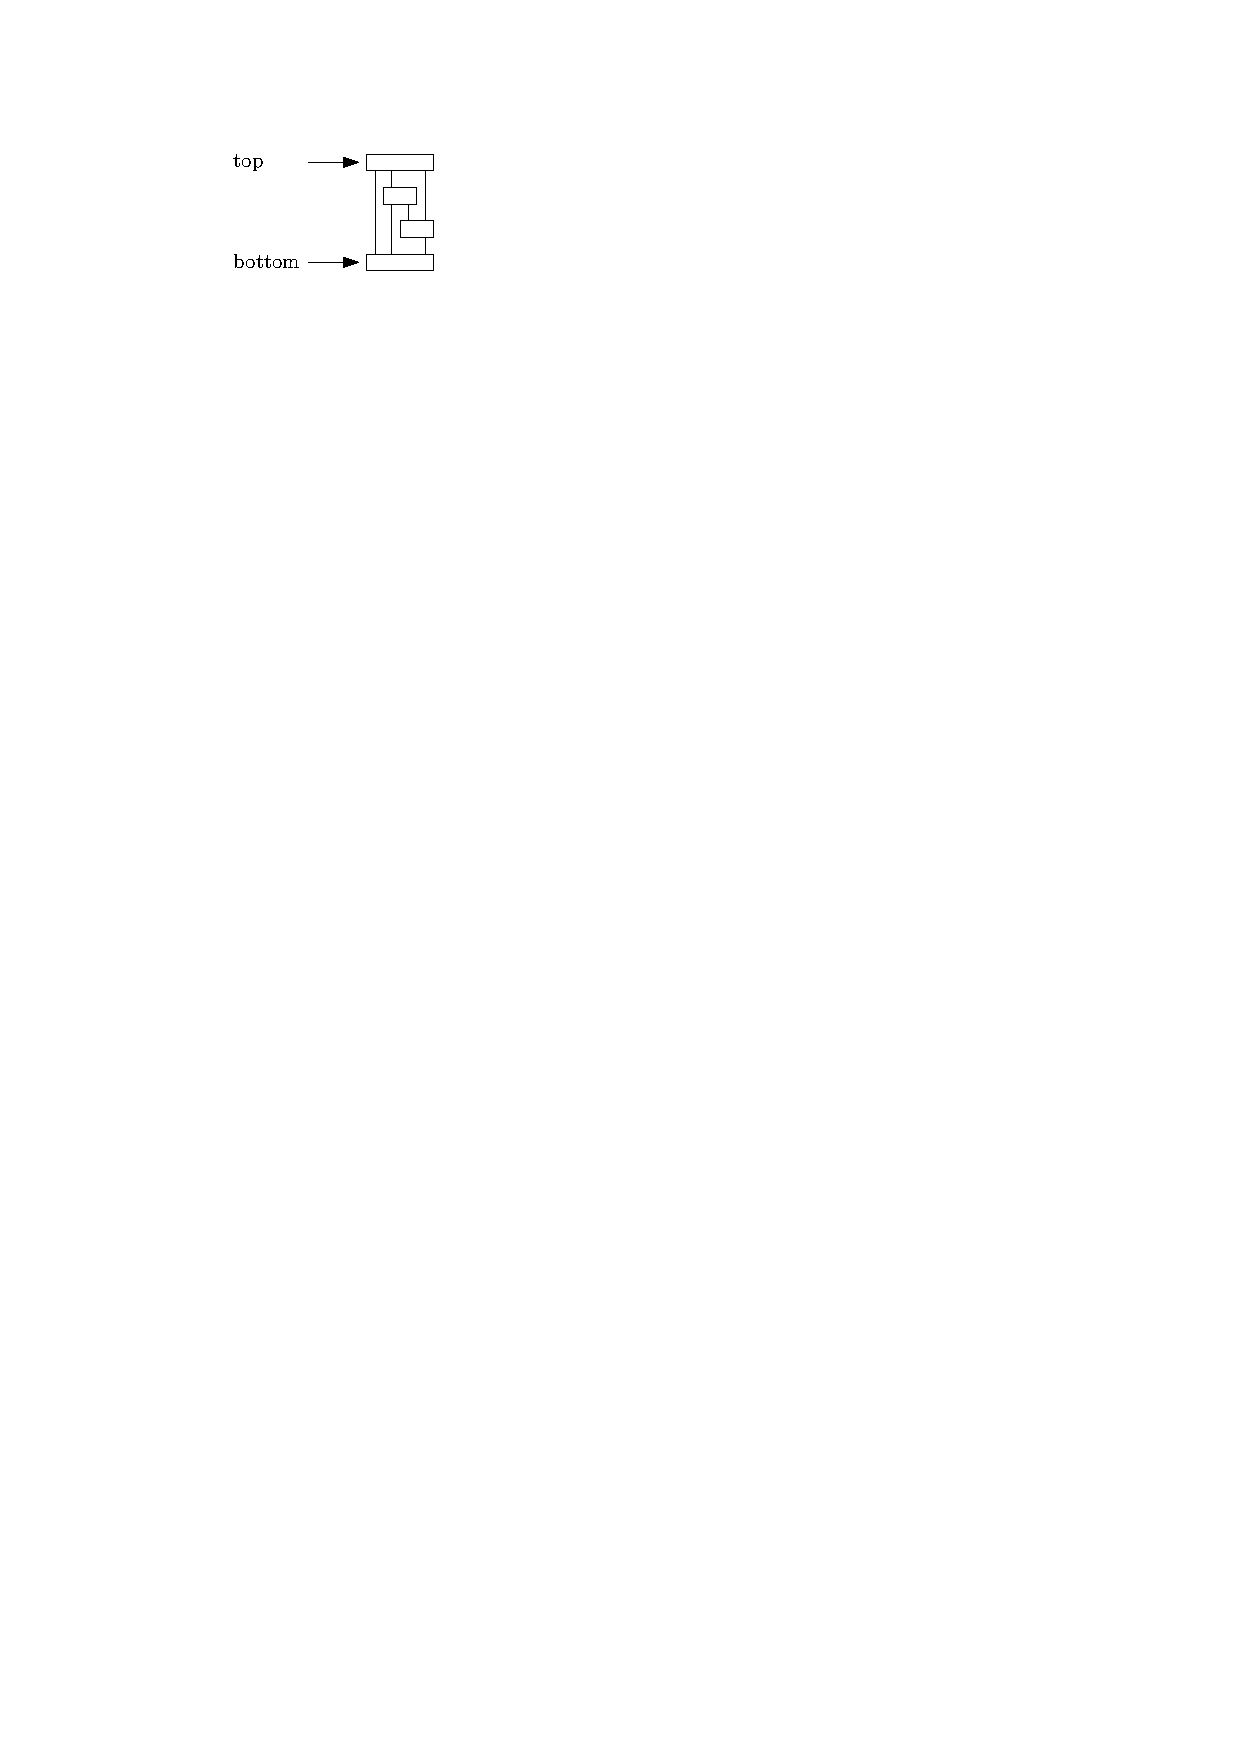
\includegraphics[page=1,width=0.4\linewidth]{graphics/3-tree_example.pdf}
	\end{subfigure}
	\caption*{$K_4$ drawn on four different layers. $\mathcal{L}_0 = (top, bottom)$}
\end{figure}

The amount of layers created while inserting vertices will determine the height of the resulting drawing.  A complete 3-tree $G$ with height $h$ in $T$ is extended to a complete 3-tree $G^+$ with height $h+1$ when for every inner face $f$ a vertex is inserted and connected to the vertices defining $f$. These newly created layers are inserted into $\mathcal{L}_h$ according to their position from top to bottom, resulting in $\mathcal{L}_{h+1}$

\begin{figure}[H]
	\centering
	\begin{subfigure}{\textwidth}
		\centering
		\includegraphics[page=2,width=0.6\linewidth]{graphics/3-tree_example.pdf}
	\end{subfigure}
	\caption*{One layer insertion in $\mathcal{B}$ when extending the height of $T$ from 0 to 1.}
\end{figure}
Let $l$ be the layer where the new vertices are inserted in according to this scheme. Every vertex insertion creates three new faces out of a pre-existing one. Unfortunately, for any layer $l$, there will be a face encapsulated between $l$ and both its predecessor and successor in $\mathcal{L}$.
\begin{figure}[H]
	\centering
	\begin{subfigure}{\textwidth}
		\centering
		\includegraphics[page=3,width=0.6\linewidth]{graphics/3-tree_example.pdf}
	\end{subfigure}
	\caption*{$\mathcal{L} = (top, l, bottom)$}
\end{figure}
So, in order to insert vertices in all the inner faces so that $G$ is a complete 3-tree and the height of $T$ will be incremented by 1, there are $|\mathcal{L}_h|-1$ at least new layers necessary.\\
For a complete 3-tree with height $h$ in its tree decomposition, the total amount of layer insertions is calculated the following way:
\begin{align*}
	&\sum_{i=0}^{h} 2^i = 2^{h+1}-1 \underbrace{\in}_{h\in \mathcal{O}(\log n)} \mathcal{O}(n)
\end{align*}
The resulting box drawing will therefore consume at least $\mathcal{O}(n^2)$ area, when the minimal distance between two layers values a constant. In conclusion, no ratio optimization is possible with this layering approach.

\subsection{Example drawing}

\begin{figure}[H]
	\centering
	\begin{subfigure}{\textwidth}
		\centering
		\includegraphics[page=10,width=0.8\linewidth]{graphics/maximal_outerplanar_example_drawings.pdf}
			\caption{Maximal SP-graph $G$ with its largest maximal outerplanar subgraph from example \ref{im:maximal_outerplanar_example_straight-line}. The differential subtrees are colored in orange}
	\end{subfigure}
	\begin{subfigure}{\textwidth}
	\centering
	\includegraphics[page=11,width=0.5\linewidth]{graphics/maximal_outerplanar_example_drawings.pdf}
		\caption{$T$ of the tree decomposition of $G$}
\end{subfigure}

\end{figure}


\begin{figure}[H]
	\centering
	\begin{subfigure}{\textwidth}
		\centering
		\includegraphics[page=12,width=0.8\linewidth]{graphics/maximal_outerplanar_example_drawings.pdf}
	\end{subfigure}
	\caption{The first differential subtree (encircled in magenta) is inserted between vertices 1 and 5 right next to the edge of $(1,5)$ (colored in cyan). Since 1 is not finished during the insertion, creating a new layer is mandatory}
\end{figure}


\begin{figure}[H]
	\centering
	\begin{subfigure}{\textwidth}
		\centering
		\includegraphics[page=13,width=0.9\linewidth]{graphics/maximal_outerplanar_example_drawings.pdf}
	\end{subfigure}
	\caption{The second differential subtree (encircled in magenta) is inserted between vertices 13 and 3 right next to the edge of $(13,3)$ (colored in cyan)}
\end{figure}